\documentclass{article}
\usepackage[left=1cm,top=2cm,right=1cm,nohead,nofoot]{geometry}

%\usepackage{times}
%\usepackage{tikz}
%\usetikzlibrary{trees}
%\usetikzlibrary{shapes,snakes}
\usepackage{verbatim}
\usepackage{amsmath}
\usepackage{amssymb}
\usepackage{setspace}
\usepackage{graphicx}

%\doublespacing

\newcommand{\R}{\mathbb{R}}
\newcommand{\Q}{\mathbb{Q}}
\newcommand{\N}{\mathbb{N}}
\newcommand{\Z}{\mathbb{Z}}
\newcommand{\qed}{\\$\Box$}
\newcommand{\qle}{\stackrel{?}{\le}}
\newcommand{\qeq}{\stackrel{?}{=}}
\newcommand{\closure}{\overline}
\newcommand{\intersect}{\cap}
\newcommand{\union}{\cup}
\newcommand{\nullset}{\emptyset}
\newcommand{\minus}{\ \backslash\ }


\begin{comment}

:Author: Micah Chambers
\end{comment}

\begin{document}
\section*{Introduction}
Functional Magnetic Resonance Imaging (FMRI) is a powerful tool in the analysis
of neural activity. Despite its rather limited temporal resolution, FMRI is still
the best way of measuring neural activity deep in the brain. 
Whereas other methods
of analyzing neural signals can be invasive or difficult to acquire, 
FMRI is relatively quick and cheap, and its analysis is straight forward.
Because of these benefits, FMRI continues to be crucial to the study of human 
cognition. Despite the fact that FMRI is so widely used,
the choice of analysis tools is still relatively limited. Every widely
available analysis tool is based on parametric modeling, which requires
prior knowledge of the noise distribution. Indeed, the linear methods
usually applied are known not to be robust to non-gaussian, non-white
noise, which is why so many pre-processing steps are necessary.
These limitations cast a long shadow over any experiment that claims to be
able to reject the null hypothesis, no matter the P-value. While obviously
there is a correlation between the BOLD signal and actual activity, its
possible the current parametric tests are over-estimating the actual amount
of activity. Its also possible that the current methods underestimate
actual activity. In this paper we propose a robust model-based approach to 
activation detection that makes no assumptions about the underlying noise
model.


fact, typical activation detection does little to account for variations
in the shape of the signal, but instead is a direct T-test between the measured signal
and the expected shape of the signal. Because of these limitations,
multiple comparison tests are imperative (ref fish), and active regions
must be very large to be detected with any confidence. This paper
will introduce a more robust method of analyzing FMRI signals for 
activation, by means of estimating the BOLD parameters.

\subsection*{FMRI}
Before going further, it is necessary to discuss Functional MRI,
and what it measures. All MRI works by exciting nuclear spin away
from a steady state controlled by a large electromagnet. Different 
nuclei respond to RF impulses based on their natural frequency
of oscillation. Therefore contrast in MRI is based on the aggregate
nuclear composition of a given region. Thus, regions with more oxygen
will respond differently from regions with proportionately less 
oxygen. This exact difference is what causes the changes over time
in the MR signal in functional MRI. Unfortunately, it takes a significant
amount of time for nuclear spin to return to equilibrium. Thus instead
of waiting, a type of imaging called Echo Planar Imaging (EPI) is used,
wherein a single excitation is used, and then as quickly as possible
every voxel (3 Dimensional Pixel) in a particular region is read. 
Because "reading" a particular region requires the switching on of a
gradient magnetic field, it takes a decent amount of time to perform
measurements. Problematically, the signal from the original excitation
drops exponentially, thus the signal to noise ratio can be very low
even at modest resolutions. Eventually the signal becomes unreadable,
and a new excitation must be applied. As more measurements are made, and thus
as the spatial resolution increases, the rate at which entire volumes
can be acquired drops. Typically volumes can be acquired every two to
three seconds, at resolutions of about 64 by 64 by 32, but their signal
to noise ratio is often poor. Other imaging modalities such as EEG and
MEG are capable of much faster measurements, but are unable to isolate
measurement locations so precisely as FMRI. As with all biological systems,
noise is much higher than in human designed systems, and yet these 
biological systems are capable of performing amazing feats.

\subsection*{BOLD Physiology}
The physiology that leads to the BOLD model has been well studied over the 
past decade and a half. While some uncertainty remains (for instance in
relation to the BOLD post-stimulus undershoot <papers relating to back and
forth on post-stimulus undershoot>) generally the model fits reality very 
well. As with every piece of tissue in the body, the brain requires oxygen
to extract energy from glucose in the blood. This process of removing oxygen
from red blood cells sets into motion a chain of events that locally 
alters the composition of the blood. Inactive neurons can be thought of
as a slingshot cocked and ready to fire. As soon as a signal moves up
the axon and causes the neuron to fire (and thus changes the state
of a membrane at that location), ions quickly move across the altered
membrane to compensate for a high charge imbalance between the interior
and exterior of the cell. This process, similar to allowing a stretched
rubber band to contract leaves the system at a lower energy state. This cannot
last though, because the neuron needs to be ready to fire again rather quickly.
To return the cell to a ready position the membrane becomes impermeable
to the ions again, and then begins pumping ions back into the cell. This
process takes a large amount of energy, whereas the actual firing takes
very little energy. Thus, after firing, glucose is burned, removing oxygen
from the blood and thus causing a dip in the ratio of oxygenated hemoglobin to 
de-oxygenated hemoglobin. This is the first potentially measurable effect
that MRI can see, although it usually lasts fewer than 2 seconds making it
difficult for FMRI to catch. As a result of the decreased amount of local oxygen,
the capillaries compensate by increasing blood flow to that region. Because,
of the quickly increased blood flow into local capillaries, the blood
volume increases in addition to the local oxygen content. This leads to a Windkessel
effect which further lags the normalization of oxygen content. The effect of
all this is an overshoot in the oxygen content above the initial level. After
the work of recharging is done, there may be a prolonged undershoot lasting
as much as 90 seconds \cite{spatial_poststim}, though the reason for this
is debated \cite{origin_poststim}. 

A large number of models have been proposed for the BOLD signal with varying
amounts of complexity. The simplest model is the so called "Balloon Model"
which first proposed the windkessel effect as a factor the BOLD response.
The model we will use is the model proposed by Buxton Et. Al. and later used
in Riera et. al. \cite{Riera}. The model has four state variables, $s$, $f$,
$v$, $q$, representing flow inducing signal, cerebral blood flow, cerebral
blood volume and deoxyhemaglobin to hemaglobin ratio, respectively. The 
state variables change over time, given by the state evolution equations:
\begin{equation}
\dot{s} = \epsilon u -  
\end{equation}

\begin{equation}
\dot{f} = s
\end{equation}

\begin{equation}
\dot{v} = 
\end{equation}

\begin{equation}
\dot{q} = 
\end{equation}

Additional papers have added such things as
....

All these effects are generally accepted as the cause of the BOLD signal, 
but FMRI doesn't detect this happening in one neuron, but rather as the 
aggregate over hundreds or millions of cells. Though local neurons act
"together" (i.e. around the same time), the density of neurons, the
density of capillaries, and slight differences in activation across 
a particular voxel can all lead to signal attenuation or noise. 
A particularly insidious type of noise present in FMRI is a low frequncey
drift, characterized by a Weiner process. Though not present in all
regions, it is prevalent enough to cause problems \cite{detrend}. It is still not
clear where exactly this noise comes although it is possible it is 
the result of magnets heating up, or some distortion in magnetic
fields. It is clear that this drift signal is not due to a true physiological
effects however, given its presence in cadavers and phantoms\cite{drift}.

\section*{Current Techniques}
\subsection*{Basic Statistical Parametric Mapping}
The most basic method of analyzing FMRI data is through a basic T-test
between "resting state" and "active state" samples. This is done by 
taking the average and variance of the inactive period, and the 
active period separately then treating them both as gaussian distributions.
If they are in fact Gaussian distributions, then a basic t-test will
give the likelihood that the samples came from the same distribution
(the p-value). Of course, this test is fraught with problems; even if
the drift mentioned earlier has been removed, there is little reason
to believe that the noise is Gaussian, or even stable. Additionally, 
even if the noise were Gaussian, a t-test with a p-value of .05 over
5000 or more samples is on average going to generate $.05*5000$ false
positives. To compensate for this, bonferoni correction, also known as
multiple comparison tests are performed; essentially p-values are 
divided by the number of independent
tests being run. This, however, leads to extremely low p-values, so
low that it would be impossible for any biological system to satisfy. To
compensate, a Gaussian kernel is applied to the image, thus reducing
variance (and thus separating the active and inactive distributions)
as well as decreasing the effective number of voxels. Since t-tests are
now no longer being applied to n <I need to define n> independent voxels,
the factor by which the p-value must be divided by can be decreased.
<Do I need to mathematically define all this?> The derivation and application
of random field theory, and its use can be found in various papers \cite{univ_mult_rft}.

\subsection*{General Linear Model}
The most used form of FMRI analysis is still based on Statistical Parametric
Mapping, but is able to account for several different levels or types
of stimulus. By adding a General Linear Model to the analysis, the
output signal timeseries (what FMRI detects) is regressed over the weighted
sum of the various confound's timeseries. The equation for a general linear
model is then
\begin{equation}
Y(t) = X(t)\beta + \epsilon(t)
\end{equation}
where $Y(t)$ is the smoothed or detrended timeseries of measurements,
$X(t)$ is a row vector of stimuli, $\beta$ is a column vector of weights,
and $\epsilon$ is the error. Thus for every time, the measurement is
assumed to be a weighted sum of the inputs plus some error. The calculation
of $\beta$ then is merely a gradient descent search to minimize the
mean squared error. 

<Image of GLM>

Of course, a square wave input is not going to result in a square wave
in the activation of brain regions. Thus, various methods are used to 
smooth $X(t)$ through time, and bandlimit the input. The best technique
is convolving the stimulus input with a hemodynamic response function,
which mimicks the basic shape of BOLD activation, including a delay
due to rise time and fall time. This hemodynamic signal is static however,
so every region of the brain gets the same design matrices (X(t)), 
although the weights of various stimulus or confounds are allowed to vary. 

<Image of Hemodynamic Response Function>

Ultimately, activation due to a particular stimuli is decided by the 
$\beta$ value corresponding to that stimuli's column of $X(t)$.
<Need to check this>
The null hypothesis as to whether the outcome was random is then
based on a t-test of the $\epsilon(t)$ timeseries. 

\subsection*{Whats wrong with these techniques}
There are a few problems with the techniques mentioned in the 
previous sections. First, they essentially ignore prior knowledge about
the system. Although the most advanced form of the general linear model includes
a "Hemodynamic Response Function," that hemodynamic response function is
static across every region of the brain. It is well known that capillary beds
are not uniform and so blood perfusion cannot possible be static across the
brain. Thus, if extra information were available a-priori, that information
could not be incorporated without modifications to the General Linear Model.
Similarly heart rate could not be added either. It would obviously be advantageous
to have true physiological parameters as entry points for these various other
model parameters. The physiological models for the BOLD signal are quite good
and based on realistic physics. While the exact connection between a stimulus
and the flow inducing signal is not precisely known, model fits are actually
quite good \cite{ModelCompareison}. Regardless, being based on some real 
physiological 
parameter would allow for the establishment of reasonable priors and decrease
model variance without breaking a sweat. Of course, using real parameters 
has the additional
bonus of potentially providing information about physical pathologies. It
is quite possible that physical properties such as decreased compliance of
blood vessels could indicate a neurological condition that is not easily
seen in a T1 or T2 map. In essence, this could make FMRI a much more 
useful clinical tool than it is now. The other problem with linear models
is that they are a linear fit to a nonlinear signal. It is not uncommon
for data to be thrown out in FMRI studies because no significant activation
has been seen. However, if, for whatever reason, the BOLD response
was acting more nonlinear than in other patients it would be completely
possible for SPM to miss that activation. 

<Image with two different $\alpha$s>

<image comparing the results of 10\% changes in various signals>

Secondly, these methods are still based on t-tests, which notoriously
lack robustness to non-Gaussian noise. While different techniques 
exist for imposing Gaussianity, those techniques are incapable of
discriminating noise from signal. There is no way to know how much 
signal is removed by various smoothing techniques, or even if entire 
regions have been smoothed into oblivion. Instead of extensively filtering data to 
remove noise, the analysis method itself must be robust a wide range of noise,
which is why we propose here the use of particle filters.

\section*{Proposed Approach}
\subsection*{Goal}
The ultimate goal of this project is to provide a new set of tools
for analyzing FMRI data. Whereas SPM techniques have been highly 
successful at finding macroscopic regions of activation, linear 
modeling can carry significant bias error due to lack of model
flexibility. While adding parameters can significantly increase
error due to model variance, this effect is mitigated by the fact
that we plan to use a model that is based on first principals. The
purpose of this paper is thus to evaluate the potential of using
a particle filter along with the BOLD model to derive physical 
parameters. In so doing, we hope to be able to show that neuronal
efficacy, $\epsilon$ is a suitable variable for estimating voxel 
activation from a standard FMRI image. We also hope to show that 
estimated posterior distribution of the parameters, derived from
the particle filter, is able to provide an accurate measure of the
confidence interval.

\subsection*{Introduction to Particle Filters}
Particle filters, also known as Sequential Monte Carlo (SMC) methods
are a powerful way of estimating the posterior probability distribution
of a set of parameters. Unlike Markov Chain Monte Carlo estimation, particle
filters extend relatively easily to any finite impulse response (FIR) system.
And unlike Variational Bayes or other gradient descent algorithms, particle
filters can be run online, with relatively lower cost. The idea of the particle
filter is to start with a wide mixture PDF of possible parameter sets, 
and then, as measurements come in, to weight more heavily parameter sets 
that tend to give good estimations of the measurements. The reliance on
an initial mixture PDF obviously introduces bias; however, it is often quite
easy to establish a reasonable range of parameters, especially when the
model being used has a physical meaning. Suppose either a set or stream
of measurements $y_t$ are made at discrete times $t = 0, 1, ... $, where
$y_t$ could be a vector of measurements. Then the goal is to find the set
of parameters $\hat{\theta}$ that give the best estimate, $\hat{y}_t$, of $y_t$.
In a biological case, with a model based on first principals, there is 
presumably some true set of parameters, $\theta$, a true model $f$
and a true observation equation, $g$ that dictate how the stimulus 
produce noisy measurements,
\begin{equation}
\dot{x}(t) = f(t, x(t), u(t), \theta) + \nu_d

y(t) = g(t, x(t), u(t), \theta) + \nu_s
\end{equation}

Where $x(t)$ is a vector of state variables, $\theta$ is a vector of system
constants, $\nu_d$ is drift noise (such as a Weiner process), $\nu_s$ is additive noise, $y(t)$ is
the vector of observations. $\nu_d$ may be driven by unknown changes in 
cerebral blood flow, or blood oxygen content, and is assumed to be zero mean.
Similarly $\nu_s$, stationary
noise could be driven by unknown changes due to the heart beat and is also assumed
to be zero mean. There are also non-biological effects that could drive these
noise terms such as inherent MR noise. 

Although not generally necessary for particle filters, we will make a few
assumptions based on the particular type of systems faced in biological 
processes. First, that $\theta$ is time invariant. This assumption is 
based on the idea that most physiological parameters don't change in the 
short run unless they are driven by some other stimulus. The obvious exception
might be something like the heart; however, period between heartbeats vary
quickly enough that accurately accounting for heart beats necessitates a 
new set of model parameters, or direct outside information. In short we
assume no parameters are time varying, because not information exists to
describe any of theme in that way. Luckily particle filters are capable 
of dealing with non-white, non-Gaussian noise, suck unanticipated influence
may be re-factored as noise. Secondly we assume that input cannot directly
influence the output, which in the case of the BOLD signal is a good assumption.
%Third, through some sort of preprocessing, we will assume that $\nu_d$ can be
%decreased or completely removed, since it 
Finally, $x(t)$ will include $\theta$, the unknown model constants, although
obviously that will mean that the vector $\dot{x}$ will always have some members
that are 0. The state space equations are then simplified to:
\begin{equation}
\dot{x}(t) = f(x(t), u(t)) + \nu_d

y(t) = g(x(t)) + \nu_s
\end{equation}

The goal of the particle filter, is then to derive the true value of $x(t)$
for each time, given known inputs $u(t), u(t-1), ... u(0)$  and noise 
measurements produced by the system, $y(t), ... , y(0)$ (every time up to
$t$). To begin with then, the particle filter starts with a prior distribution,
which is used to build a Dirac Mixture Probability Distribution function:

\begin{equation}
P(\hat{x}(0)) = \frac{1}{N}\Sigma_0^{N-1} \delta(x_(0) - \hat{x}_i(0))
\end{equation}

where $\hat{x}(0)$ is an empirical representation of the prior, and $\hat{x}_i(0)$
is the $i^{th}$ particle, a single possible representation of the system at time 0.
Initially, since each $\hat{x}_i$ has been drawn form the prior, and no measurements
have been made, the particles are all equally weighted. When a measurement becomes
available, that information is then incorporated into the posterior by re-weighting
the particles .

\begin{equation}
\dot{y} = -ky
\end{equation}
$\theta_i$ would have an estimate for $k$ \emph{and} $y$. Of course in many cases
the model is a potentially non-linear differential equation with no closed
form solution. Initially every $\theta_i$ will have the same weight, because
there isn't yet anything to base a weighting on. Note that this doesn't mean
that the particles have been evenly distributed, so the distribution is not 
necessarily "flat" just because all the particles are equaly weighted. When a
new measurement is available, the particles are then reweighted based on how
well they predicted the new measurement. 

\subsection*{My Specific Particle Filte}
Although particle filters are well defined, significant design decisions
are application dependent. The most important choice is the weighting function,
$w(y_t - y(\theta_t))$. Obviously the function should weight $0$ maximally,
the drop off rate is extremely important. A very thin gaussian probability 
distribution function has nice properties, but thin tails. As a result, large
outliers in the measurement vector could easily force all the particles to
have near 0 weights, thus forcing the particle filter to converge improperly. 
On the other end of the spectrum, a cauchy pdf may not
weight particles in the middle enough, preventing the particles to never 
converge. Of course, the scale factor, or variance, also plays a signifcant
role in the convergeance rate. The importance of the weighting function
cannot be overstated, as this is the primary factor in deciding the rate at
which the particle filter converges. As part of the simulations, I compare
a gaussian based weighting function with an exponential weightin function.
In both cases, I scaled the width of the weighting functions automatically based
on the signal variance.

Dealing with low frequency noise is also a crucial part of the tests. 
I tested two different methods of dealing with this noise. Various methods
are used to deal with this problem in other toolsets. The most common method
is to apply a high-pass filter to the measurement vector. Although this makes
sense in many applications, in this case it may not be adaptive enough for
a random walk type noise. On the other hand, it has been shown that a spline
de-trending method is able to better deal with the low frequency noise
typically present in FMRI. Thus, my first method
was to use a spline fit with knots every 80 or 90 measurements to trance
the basic shape of the drift. I then added an extra DC gain parameter to
the model to account for the fact that the de-trended signal tended to have 
a mean of 0, rather than some positive value. 

My second method of dealing with low frequency drift was to counteract
it by weighting particles based on $(y_t-y_{t-1}) - (y(\theta_t)-y(\theta_{t_1}))$ 
rather than directly on $y_t - y(\theta_t)$. It is generally believed that the noise present in 
FMRI has approximately gaussian steps, which means that this method only
has to deal with gaussian white noise. Such a technique is usually not considered a
good idea because high frequency noise is almost exclusively assumed in
systems theory. In this case however; the noise is all in the lower frequency
range, so performing a differentiation like operation, which magnifies high
frequency signals, is exactly what we want. 

... more specifics...

The General Linear Model, and 
SPM's goal is to find a correlation between input, or what a 
person is thinking, and which regions are active. This is an 
important task, but it misses the potential of FMRI. FMRI's 
greatest weakeness as a tool for studying neural activity is that
it is connected to neurons through a long chain of events. But
what if, in addition to seeing which brain regions are active
for which stimuli, we could also study pathologies such as poor
blood flow, or derive physical parameters such as blood vessel
compliance? By using a realistic physical model as the basis for
discovering the relation between the outside world and FMRI 
signal, the path to detecting activation gives all those other
things for free, precisely \emph{because} FMRI is the result of such
a long chain of events. It is actually quite common to use models to derive
the values of physiological parameters. For instance, blood volume
is often measured by injecting a dye into the blood stream and then
assuming that the dye is removed at a rate proportional to the
concentration in the blood. By performing a simple regression it is
possible to estimate blood volume quite accurately. While for
this particular project I don't claim that the results will give 
physiologically plausible results, with some tuning of the algorithm
it would very possible. 

While the General Linear Model has historically done well with
detecting activation, it is limited to scaling the entire input
signal up or down. This leaves out even basic effects such as 
longer or shorter time constants, as well as nonlinear effects which
are known to be present in the BOLD system. 
**


While the General Linear Model has been extremely effective at
gleaning information about which voxels are "active" and which
are not, its purpose is only to say which regions are "statistically
significant". However, considering that voxels consist of millions
of neurons, the reality is that a
region could be active, but at some other level or time constant
than expected; and be completely missed by the linear model. 
Studies showing activation
in Cadavers of Phantoms highlight the inherant problem with the 
General Linear Model: a problem that mandates multiple
comparison testing with very high thresholds to ensure any 
sort of face validity \cite{drift}.
By moving to models that actually "learn" the 
parameters of the model, model error will be drastically
reduced allowing for much more reasonable statistical thresholds.
\subsection{Particle Filters}

\section*{Methods}
\subsection*{Preprocessing}
After FMRI data has been acquired it is always necessary to modify the
data in some way to make different runs comparable. Because FMRI signal
levels are essentially unit-less, at the very least it is necessary to convert
the data into \% difference from the baseline. Finding the baseline is the
first hurdle in dealing with FMRI. Various methods exist for doing this,
but they are all ad-hoc. It is common to treat each stimulus pulse independently,
ignoring the long decay of the BOLD signal. By treating each input separately,
the "base" for calculating the percent difference is merely the signal level 
before the stimulus is applied. The problem with this is that the BOLD signal
can be heavily delayed, and fall times can be as long as 10 or 15 seconds,
meaning that the assumption is clearly a false one. Another popular method 
of dealing with this problem, is to put all the time series through a high
pass filter. This will of course remove the DC component of the signal, and 
some amount of so called "drift". The problem with this method is that it is
not adaptive to the input. Huge variations in drift frequencies can exist 
in a single time-series. Thus, a single cutoff frequency could miss a significant
drift component, or it could remove \emph{actual} signal, if the cutoff frequency is
set too high. 


\section*{Introduction to Modeling}

Of course, it is well known that many of the assumptions 
that the GLM makes about BOLD activation do not hold. 
The General Linear Model ignores
the fact that the BOLD response is nonlinear, contains non-gaussian
noise and most importantly that brain networks are 
so called "Small World Networks" \cite{smallworld}, \cite{noise}. 
Merely accounting for
nonlinearities in the time-series of the BOLD response can
result in significantly better estimation as shown in \cite{nonlinearmodels}.
But even more crucial is the recent movements away from mass-
univariate models. Current mass-univariate models 
assume uniform connectivity from input to every voxel; yet
this is obviously not the case. While
violating linearity assumptions or Gaussian assumptions 
requires us to be more conservative, the lack of any method
to switch brain circuits on and off means that any model
we make for brain regions would not be Turing complete;
in effect implying that humans are incapable of 
thought \cite{turing}.

So called Dynamic Causal Modeling is the beginning of 
the next phase of neurology. DCM is the first 
brain study to show any significant connection between 
diffusion tensor imaging and actual function layout in
the human brain \cite{dti_dcm}. By incorporating connections
between regions and a realistic activation model, DCM
corrects two of the largest problems with the GLM. While
there are other techniques that may be useful in the future,
they either lack physiological analogs (Artificial Neural
Networks) or are extremely computationally expensive 
(mutual information).  Given that much of the 
potential of the GLM has been exhausted, and that DCM 
is one of the first well defined methods capable of learning 
complicated brain circuits DCM is crucial to the future
of FMRI and our understanding of the human brain.

\section*{Results}
The particle filter shows great promise in being able 
to learn a variety of different regional activation
parameters. We have performed tests with a random binary
pulse train as input to a simulated region and then tested
the particle filter's ability to estimate the signal
parameters. Additionally random gaussian noise with an
Signal-To-Noise ratio of 2.0 was added. Figure 1 shows
the pulse train, the clean signal and the noisy signal, which
was the input to the particle filter. A random set of 
system parameters was chosen to simulate the region,
which the particle filter had no knowledge of other than
a mean and rough variance.
The tests were performed using 10,000 particles and took
approximately 4 minutes to compute.

%figure 1
\begin{figure}
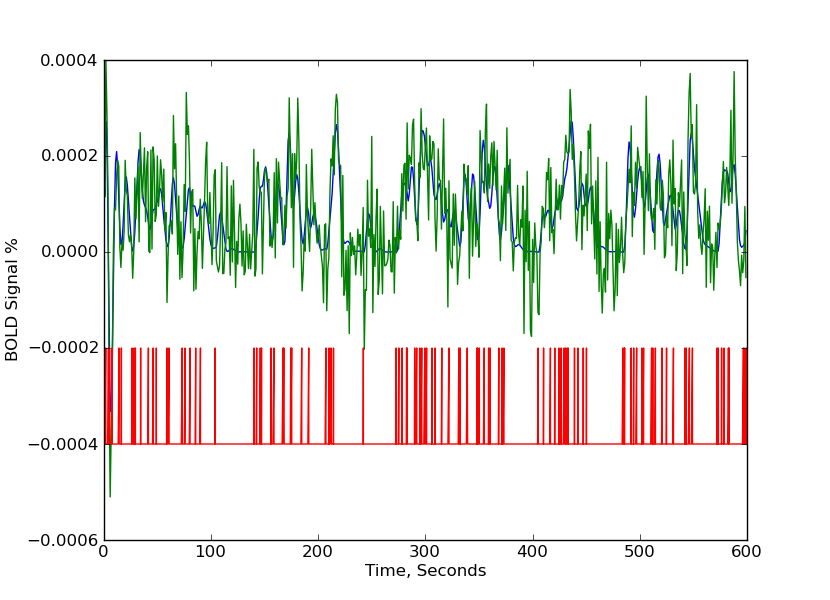
\includegraphics[width=8in,height=4in]{noise.png}
\caption{Simulated time-series for a single region. The red line
shows the input stimulus, the blue line shows the base BOLD 
response, and the green line is the BOLD response with Gaussian
white noise added at SNR of 2}
\label{fig:noise}
\end{figure}

%figure 2
\begin{figure}
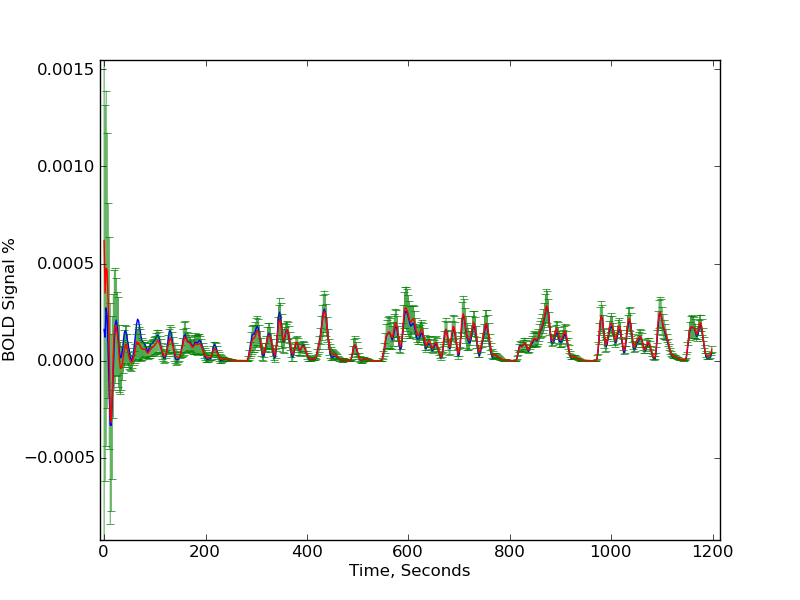
\includegraphics[width=8in,height=4in]{bold.png}
\caption{Particle Filter Results. The blue line is the "true"
(simulated) BOLD response, the red line
is the output of the particle filter with 2 standard deviations
in green. Note that the error bar for time 0 is outside the scope
of the image and is approximately $\pm .003$.}
\label{fig:bold}
\end{figure}

%figure 3
\begin{figure}
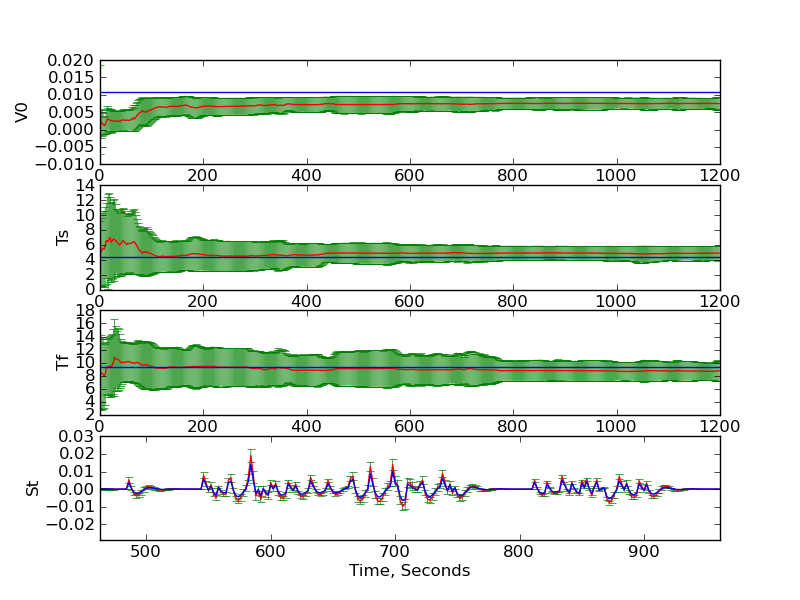
\includegraphics[width=8in,height=4in]{state.png}
\caption{Particle Filter Results. The blue line is the "true"
parameter and the green line is the estimated value for the parameter.
Note that the timescale for $S_t$ is different to highlight an typical
stimulus response. Again 2 standard deviations are shown.}
\label{fig:state}
\end{figure}

Figure 2 shows the estimated BOLD response versus the simulated
data (without noise). It is clear that as the estimated BOLD
response converges to the true BOLD as time progresses. This
is because more and more potential states are eliminated by system's
response to new input sequences. Convergence depends highly on 
the input signal and the weighting function thus choice of both
are extremely important. We have found that an impulse train
(emulated with .1 second width square waves) gives a very good
response. It is also important to choose an input with
some longer hold times, at least as long as than the 
expected time constants, which in this case was around 
8 seconds. The weighting function we have chosen is based
on the exponential distribution, with a variance equal to
the RMS of the signal. While it is important to converge
by the end of the time-series, it is often the case that 
converging too fast will harm the state estimation by over-
emphasizing the measurements of single time points. The rate
of convergence is well within control of the user of the 
particle filter based on the weighting function and the frequency
of re-sampling. Note that resampling can cause quantization
errors due to the nature of estimating a long tailed 
distribution with a finite number of samples. 

Figure 3 shows the estimated versus simulated values for
several key parameters. Notice how the variance drops as
the particle filter continues. The parameters shown are
$V_0$ which is a scaling parameter, $\tau_s$, and $\tau_f$
which are both time constants and $s_t$ which is a hidden
state variable, estimating the flow inducing signal. Note that
even though some of the parameters don't converge to the exact
value, that the estimated $s_t$ still matches the true
$s_t$ relatively well. It is often the cast that although a
few parameters don't converge to their true value, one 
parameter may pick up the slack for another. It is of
note that $\tau_s$ and $\tau_f$ do converge at least close
to their true values, because they cannot be determined
from steady state. 

\bibliographystyle{abbrvnat}
\bibliography{proposal_micah}


\end{document}
